\documentclass[11pt]{article}
\usepackage[document]{ragged2e}
\usepackage[letterpaper, margin = 1in]{geometry}
\usepackage[utf8]{inputenc}
\usepackage{parskip}
\usepackage{circuitikz}
\usepackage{mathtools}
\usepackage{graphicx}
\usepackage{amsmath}
\usepackage{physics}
\usepackage{epstopdf}
\usepackage{indentfirst}
\usepackage{multicol}
\setlength{\columnsep}{1cm}
\usepackage{wrapfig}
\usepackage{subcaption}
\usepackage{siunitx}

\begin{document}
\centering
\textit{Summer Research 2019 Notes}\\
\textbf{Direct application of Bayesian inference on dynamic light scattering experiments to infer discretized particle size distribution}\\
Thy Doan Mai Le

\justifying
\section{Introduction}
Write about dynamic light scattering, why we're doing this, applications, what I'm trying to do specifically, previous works by other groups

\section{Testing Notes}
With an implementation of the $g^{(2)}$ function, a Gaussian distribution, a bidisperse distribution as well as a single point distribution of particle sizes were used to test the validity of the $g^{(2)}$ function's implementation. 
\subsection{Bidisperse Distribution}
The following self-generated particle size distribution with two peaks of different full-width-half-max (FWHM) values was used to test the validity of the $g^{(2)}$ function on a bimodal distribution. The reason for this test is to verify that the implementation written is able to work with a bimodal size distribution, since one of the advantages of the Direct Bayesian Method (DBM) is that it is able to work with almost any particle size distribution. 

\begin{figure}[h]
\centering
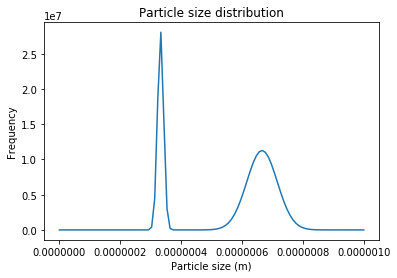
\includegraphics[width=0.5\linewidth]{bidisperse_psd.png}
\caption{The distribution of particle size (not normalized here) has a peak at $3.33\times10^{-7}$\si{meter} and another peak at $6.66\times10^{-7}$\si{meter}}
\label{fig:bidisperse_psd}
\end{figure}

From this distribution, the $g^{(2)}$ autocorrelation function of intensity v. time was found to be:

\begin{figure}[h]
\centering
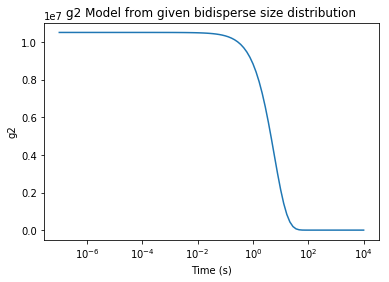
\includegraphics[width=0.5\linewidth]{g2.png}
\caption{The $g^{(2)}$ autocorrelation function extrapolated from the implementation.}
\label{fig:g2_model}
\end{figure}

In order to verify the validity of this autocorrelation function, I used SciPy's optimization for curve fits to extrapolate, from this autocorrelation function, the single exponential decay and the method of cummulants models. The goal of this method of testing is to verify that both of the single exponential decay and cummulants models fail upon the emergence of a bimodal particle size distribution. In order to detect this anticipated failure, the residuals between the $g^{(2)}$ model and each of the tested models (single exponential/cummulants) are plotted. Failure of each of the tested models is present when overshooting and/or undershooting are present in the residuals plot. 

When tested against the single exponential decay model, the residuals plot is as follows:

\begin{figure}[h!]
\centering
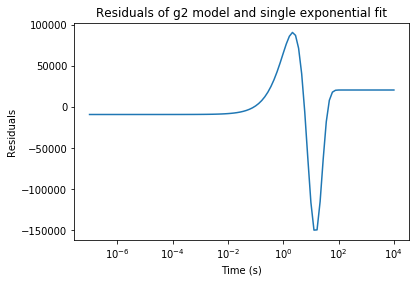
\includegraphics[width=0.5\linewidth]{expo_residuals.png}
\caption{The undershooting and overshooting are both apparent around the region of exponential decay, implying that the exponential fit is unable to capture certain aspects of the autocorrelation. This is congruent with the given data. Since single exponentials are only able to capture information of systems with 1 single particle size, a bimodal distribution of particle size should render the single exponential model inept.}
\label{fig:expo_residuals}
\end{figure}

When tested against the cummulants model, the residuals plot is as follows:

\begin{figure}[h!]
\centering
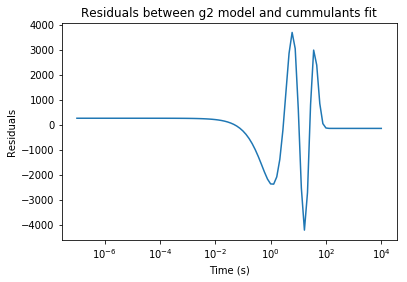
\includegraphics[width=0.5\linewidth]{cummulants_fit_residuals.png}
\caption{The residuals between the autocorrelation and the cummulants fit model showed dramatic breakdown around the exponential decay region, signifying that the cummulants fit was not able to truly capture the $g^{(2)}$ information.}
\label{fig:cummulants_residuals}
\end{figure}

In conclusion, the residuals plots have shown that both the single exponential and the cummulants model were unable to fully capture the information displayed in the $g^{(2)}$ autocorrelation and therefore should not be used in analyzing dynamic light scattering information of samples with know multimodal particle size distributions. 

\subsection{Single Gaussian distribution}

\section{Derivation of Bayesian distributions}
\subsection{Prior Distribution}
According to Buoalem, Jabloun, Ravier, Naiim and Jalocha, the prior distribution of this non-parametrized method is as follows:
\begin{equation}
p(\mathbf{f}) \propto exp\left( \mathbf{f}^{T} \mathbf{L_2}^{T}\mathbf{L_2}\mathbf{f} \right), \textrm{if } \mathbf{g} \geq 0
\end{equation}

\subsection{Likelihood Distribution}
The likelihood distribution is modeled according to the $g^{(2)}$ function as 

\begin{equation}
p(\mathbf{\sim{g^{(2)}}} | \mathbf{f}, \sigma^{2}_r ) = \frac{1}{{(2\pi)}^{\frac{M_r}{2}} \sigma^{M_r}}exp\left( -\frac{\chi_r(\mathbf{g})}{2\sigma^2_r}\right)
\end{equation}
if the 
\end{document}